% Matthew Monaco
% Andy Sayler
% Landon Spear
% University of Colorado
% Networked Character devices
% Fall 2011

\documentclass[11pt,twocolumn]{article}

\usepackage[text={6in, 9in}, centering]{geometry}
\usepackage{graphicx}
\usepackage{url}
\usepackage{listings}

\bibliographystyle{plain}

\lstloadlanguages{C}
\lstset{
  language=C,
  basicstyle=\footnotesize,
  numbers=none,
  numberstyle=\footnotesize,
  stepnumber=1,
  numbersep=5pt,
  showspaces=false,
  showstringspaces=false,
  showtabs=false,
  tabsize=4,
  captionpos=b,
  breaklines=true,
  breakatwhitespace=false,
  title=\lstname,
  frame=single,
  frameround=tttt
}

\newenvironment{packed_enum}{
\begin{enumerate}
  \setlength{\itemsep}{1pt}
  \setlength{\parskip}{0pt}
  \setlength{\parsep}{0pt}
}{\end{enumerate}}

\newenvironment{packed_item}{
\begin{itemize}
  \setlength{\itemsep}{1pt}
  \setlength{\parskip}{0pt}
  \setlength{\parsep}{0pt}
}{\end{itemize}}

\begin{document}

\title{Networked Character Devices}
\author{Monaco, Matthew \and Sayler, Andrew \and Spear, Landon
  \\ \and University of Colorado}
\date{\today}

\maketitle

\begin{abstract}
While there are various projects which provide a network abstraction layer for
specific high-level subsystems in the Linux kernel, there aren't any low-level
general purpose solutions. Network character devices (NCD) is a system for
exporting character device drivers of a fast, local network. However NCD works
to some extent with regular files, block devices, sockets, and pipes; it is also
suitably responsive over Internet connections for many applications.
\end{abstract}

% Landon Sections

\section{Introduction}
\label{sec:introduction}

We did some stuff, we used some references \cite{ldd3}.

\section{Related Work}
\label{sec:relatedwork}

We are unique.

% Matt Sections

\section{Architecture}
\label{sec:architecture}

\begin{figure}[h]
  \begin{center}
    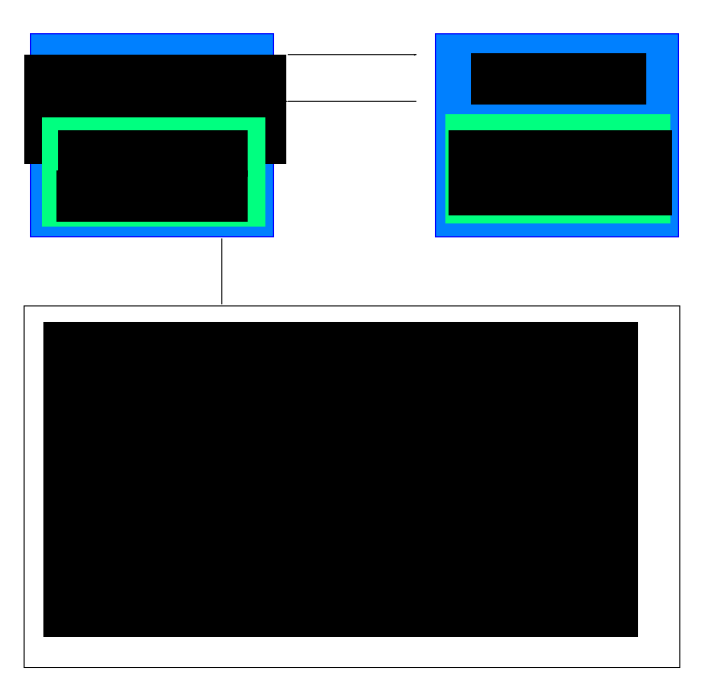
\includegraphics[width=0.5\textwidth]{arch-03.png}
  \end{center}
  \caption{The basic client-server model of NCD.}
  \label{fig:architecture}
\end{figure}

On a very high level, NCD uses a basic client server model. The client
issues a request to the server, which in turn issues a reply. The
server never initiates any communication on its own.

\subsection{Client}

The client is currently implemented entirely within an out-of-tree kernel
module. This is arguably not the most robust, nor secure, solution. See
section \ref{sec:futurework} for details on splitting out some functionality
into a user-space helper.

Devices which have been imported on the client reside within the
devtmpfs filesystem. This is almost always mounted on \texttt{/dev}. By
default an imported device will take on the name
\texttt{/dev/netchar/importN}, where \texttt{N} is the next available
number. In the future (and without much effort), imported devices will
be able to take on their original name from the server. For example, an
input device can be located at \texttt{/dev/input/eventN}. Furthermore,
the user or administrator may choose any mapping (s)he see fits.

\subsection{Server}

The server is, as mentioned, a typical user-space daemon. It
currently only services a single file. Whether or not the server should
handle multiple exports is still up for evaluation.

The server listens on a port specified on the command line. There is no
default. When a request is received from the client, it will correspond
to one of the standard VFS file operations. Currently, \texttt{open()},
\texttt{close()}
\footnote{The counterpart for \texttt{close()} is actually referred to
as \texttt{release()} within the kernel.}
, \texttt{read()}, and \texttt{write()} are supported.

After receiving a request, the server then performs the requested
operation locally and returns the result to the client in a reply
message. For example, if the client sends an \texttt{open()} request,
the server will open and hold a file descriptor on the client's behalf.

This straightforward architecture will actually support any file type
(with certain restrictions for each type). Character devices, regular
files, sockets, and pipes should work fully (when all file operations
are implemented). Block devices and even directories will work to some
extent.

\subsection{Protocol}

\begin{figure}[h]
  \begin{center}
    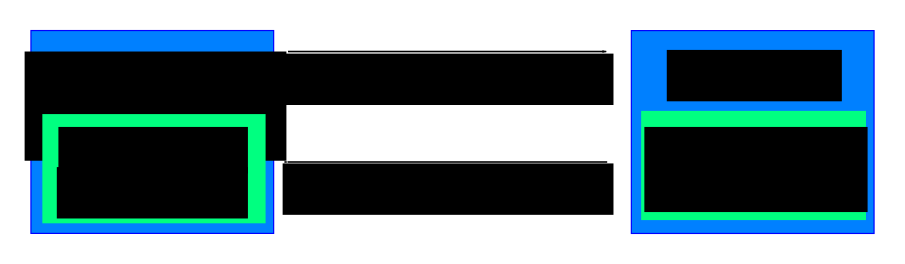
\includegraphics[width=0.5\textwidth]{proto.png}
  \end{center}
  \caption{NCD operates over a simple request reply protocol. Bulk data
  immediately follows formal messages, as required.}
  \label{fig:protocol}
\end{figure}

The protocol is implemented as a simple request-reply system over
\texttt{INET} sockets. All request types are encapsulated within a
single request structure (see section \ref{sec:implementation}).
Similarly, there is only a single reply structure to account for all
reply types.

Bulk data is sent in the raw immediately following the corresponding
request/reply. In the case of a \texttt{read()}, the targeted data
immediately follows the reply. In the case of a \texttt{write()}, the
targeted data immediately follows the initial request.

\section{Implementation}
\label{sec:implementation}

% Andy Sections

\section{Results and Evaluation}
\label{sec:results}

The Network Character Device system is still a work in
progress. We will need to Expand the system beyond it's current state
before the NCD concept is ready for production-level use.

Non the less, we have gained many insights into the advantages such a
system might provide. We have also encountered the difficulties
implementing such a system into an existing OS like Linux entails.

\subsection{Current Status}
\label{sec:currentstatus}

As of this writing, we have completed a partial implementation of
the Network Character Device system. Current functionality includes:

\begin{packed_item}
\item Support for exporting a single character device from the server
\item Support for importing a single character device on the client
\item Client-side kernel-space Linux module implementation
\item Server-side user-space background process implementation
\item Support for open, close, read, and write calls
\item Basic Linux udev support for automatic node creation on client
\end{packed_item}

This set of core functionality provides a working proof-of-concept
Network Character Device system. This system fully supports the
export of a single character device from server to client over the
network and demonstrates the basic use and utility of such a system.

It should be noted, however, that some work is still required before
the Network Character device system can be considered a production
ready utility. Most notably, the following features are necessary for
a fully functional NCD system, but are not yet included in our
implementation:

\begin{packed_item}
\item Multi-device, multi-server client-side import support
\item Multi-device server-side export support
\item Support for exclusive use and protection of exported devices
\item Support for ioctl calls
\item Support for providing and obtaining metadata for exported
  devices
\item Support for ``advertisement'' of available exported devices
\item Support for integrating imported devices into other kernel
  subsystems (human interface subsystem, audio subsystem, etc)
\item Addition of ``NCD-admin'' utilities for managing and administering
  NCD system
\end{packed_item}

Section \ref{sec:futurework} provides some insight into the addition
of some of these expanded features.

\subsection{Advantages}
\label{sec:advantages}

\subsection{Challenges}
\label{sec:challenges}

\section{Future Work}
\label{sec:futurework}

\section{Conclusion}
\label{sec:conclusion}

\bibliography{refs}

\end{document}

% vim: set ts=2 sts=2 sw=2 et spell tw=72 : %
